% !TEX program = pdflatex
% !TEX options = -synctex=1 -interaction=nonstopmode -file-line-error -shell-escape "%DOC%"

\documentclass[crop,tikz,convert={outext=.svg,command=\unexpanded{pdf2svg \infile\space\outfile}},multi=false]{standalone}
\usetikzlibrary{shapes,backgrounds,decorations.pathreplacing}
\usepackage{amsfonts,amssymb,amsthm,amsmath}

\definecolor{mycolor1}{RGB}{27,158,119}
\definecolor{mycolor2}{RGB}{217,95,2}
\definecolor{mycolor3}{RGB}{117,112,179}


\begin{document}
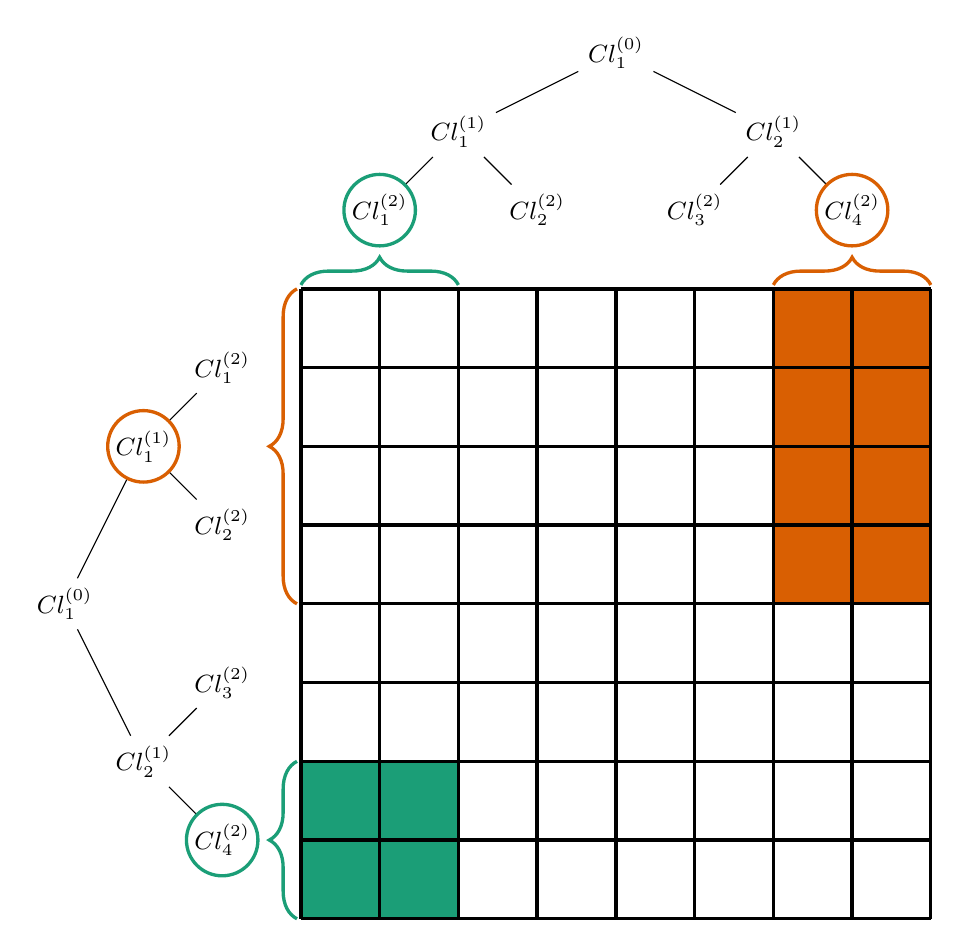
\begin{tikzpicture}
    \tikzstyle{every node}=[font=\small]

    % Matrix
    \draw[very thick] (0,0) grid (8,8);

    % Source tree
    \node at (4,11) (Is00) {\(Cl^{(0)}_1\)} ;
    \node at (2,10) (Is10) {\(Cl^{(1)}_1\)} ;
    \node at (6,10) (Is11) {\(Cl^{(1)}_2\)} ;
    \node[circle, draw=mycolor1, very thick, inner sep=1pt] at (1,9) (Is20) {\(Cl^{(2)}_1\)} ;
    \node at (3,9) (Is21) {\(Cl^{(2)}_2\)} ;
    \node at (5,9) (Is22) {\(Cl^{(2)}_3\)} ;
    \node[circle, draw=mycolor2, very thick, inner sep=1pt] at (7,9) (Is23) {\(Cl^{(2)}_4\)} ;

    \draw (Is00) -- (Is10);
    \draw (Is00) -- (Is11);
    \draw (Is10) -- (Is20);
    \draw (Is10) -- (Is21);
    \draw (Is11) -- (Is22);
    \draw (Is11) -- (Is23);

    % Target tree
    \node at (-3,4) (It00) {\(Cl^{(0)}_1\)} ;
    \node at (-2,2) (It10) {\(Cl^{(1)}_2\)} ;
    \node[circle, draw=mycolor2, very thick, inner sep=1pt] at (-2,6) (It11) {\(Cl^{(1)}_1\)} ;
    \node[circle, draw=mycolor1, very thick, inner sep=1pt] at (-1,1) (It20) {\(Cl^{(2)}_4\)} ;
    \node at (-1,3) (It21) {\(Cl^{(2)}_3\)} ;
    \node at (-1,5) (It22) {\(Cl^{(2)}_2\)} ;
    \node at (-1,7) (It23) {\(Cl^{(2)}_1\)} ;

    \draw (It00) -- (It10);
    \draw (It00) -- (It11);
    \draw (It10) -- (It20);
    \draw (It10) -- (It21);
    \draw (It11) -- (It22);
    \draw (It11) -- (It23);

    % Blocks
    \begin{scope}[on background layer]
        \fill[mycolor1] (0,0) rectangle (2,2);
        \fill[mycolor2] (6,4) rectangle (8,8);
    \end{scope}

    % Braces
    \draw [decorate,decoration={brace,amplitude=10pt},very thick,mycolor1] (-0.05,0) -- (-0.05,2);
    \draw [decorate,decoration={brace,amplitude=10pt},very thick,mycolor1] (0,8.05) -- (2,8.05);

    \draw [decorate,decoration={brace,amplitude=10pt},very thick,mycolor2] (-0.05,4) -- (-0.05,8);
    \draw [decorate,decoration={brace,amplitude=10pt},very thick,mycolor2] (6,8.05) -- (8,8.05);

\end{tikzpicture}
\end{document}
